% Preamble
% ---
\documentclass{article}

% Packages

\usepackage{graphicx}
\usepackage{subfig}
\usepackage{pgfplots}

\usepackage{multicol}
\usepackage{float}

\usepackage{tikz}
\usetikzlibrary{shapes.geometric, arrows}

\usepackage[english]{babel}

\usepackage{geometry}
\geometry{margin=1.2cm}

% ---


\graphicspath{ {assets/} }

\setlength{\columnsep}{1.3cm}
\begin{document}

\setlength{\columnsep}{0.8cm}
\begin{multicols}{2}

\section{Introduction}

This report will evaluate the Viola-Jones detector as a frontal face detector and dartboard detector. It will then build on the Viola-Jones detector to improve its recall and precision.

\section{Face detection}

% -- Part 1 - Image section
\setlength{\columnsep}{0.1cm}
\begin{multicols}{2}
  \centerline{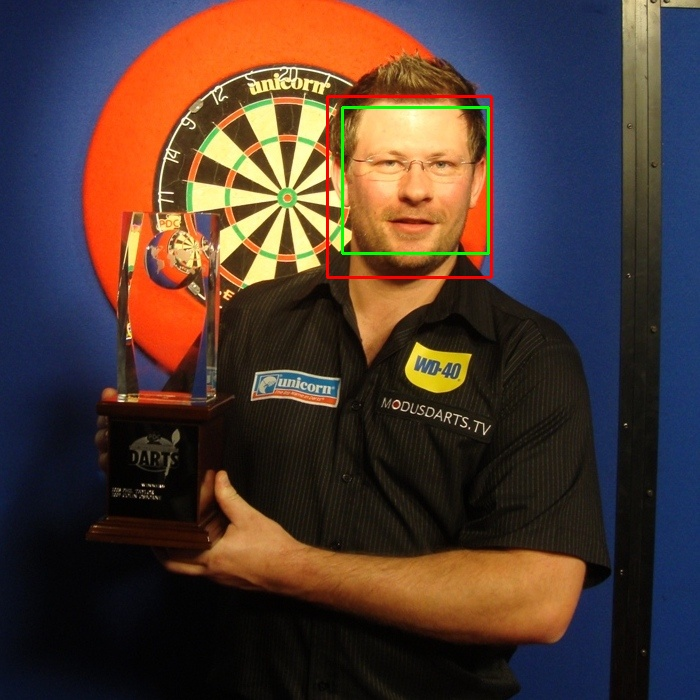
\includegraphics[width=\linewidth]{dart4-face.jpg}\par}
  \centerline{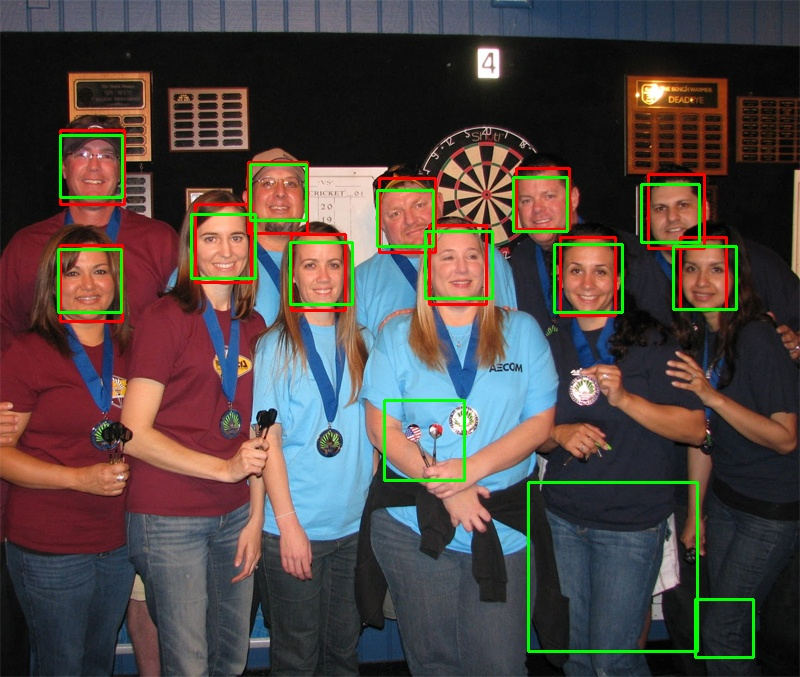
\includegraphics[width=\linewidth]{dart5-face.jpg}\par}
  \centerline{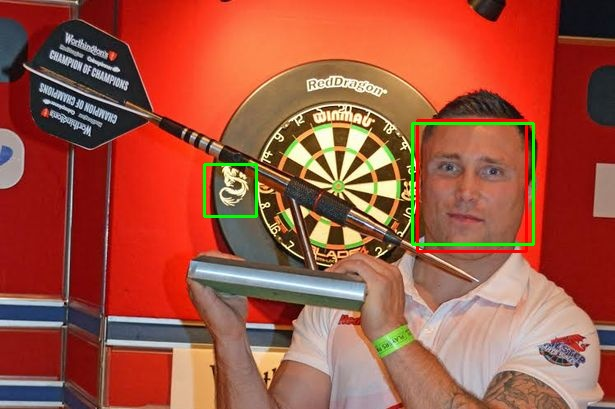
\includegraphics[width=\linewidth]{dart13-face.jpg}\par}
  \centerline{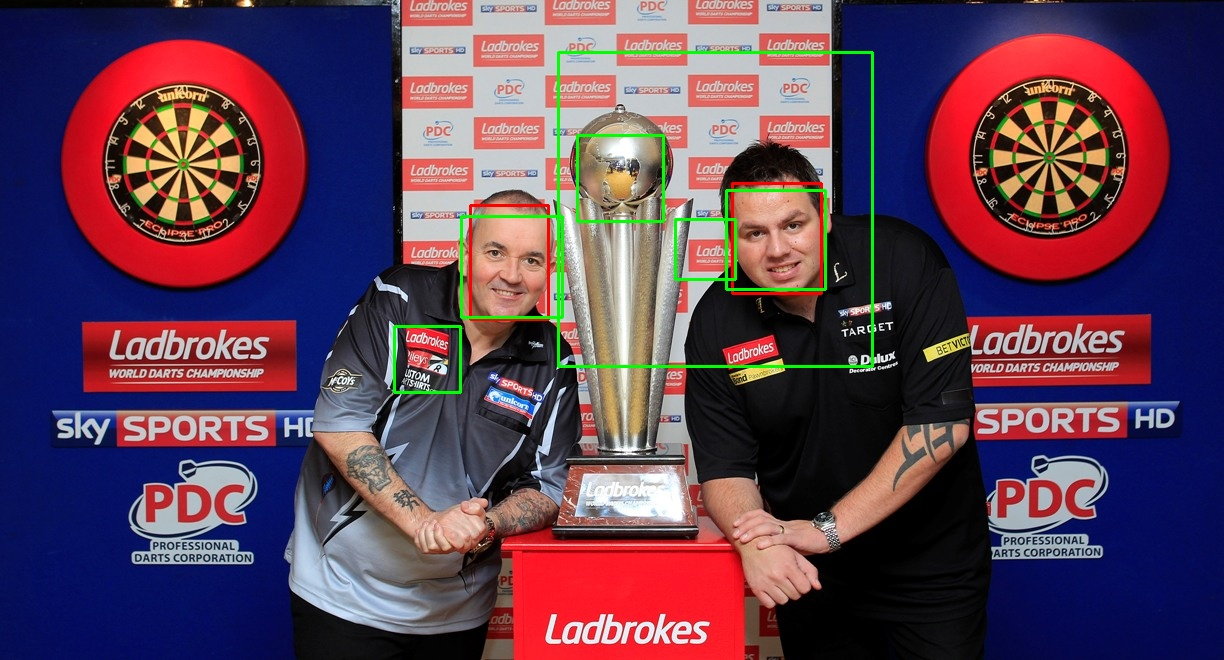
\includegraphics[width=\linewidth]{dart14-face.jpg}\par}
  \centerline{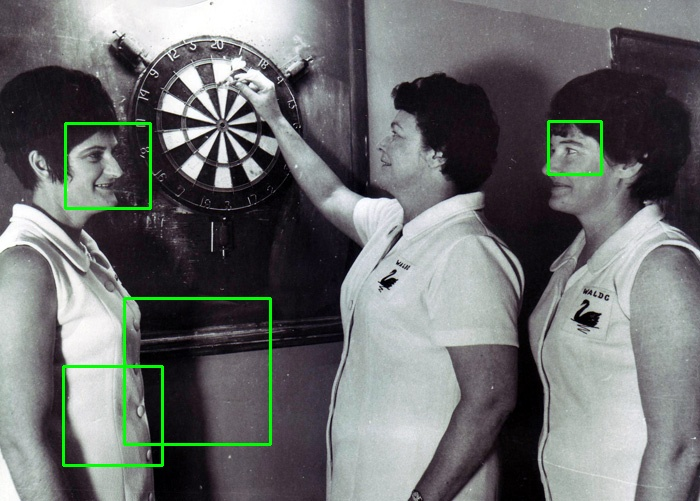
\includegraphics[width=\linewidth]{dart15-face.jpg}\par}
\end{multicols}
\captionof{figure}{Viola-Jones face detection (green) with ground truth (red)}
\label{fig:vjfaceimages}

\begin{center}
\begin{tabular}{ |p{2cm}||p{2cm}|p{2cm}| }
 \hline
 \multicolumn{3}{|c|}{Frontal face detection results} \\
 \hline
 Image name & TPR & F1-SCORE \\
 \hline
 dart4  & 1   & 1         \\
 dart5  & 1   & 0.88      \\
 dart13 & 1   & 0.666667  \\ 
 dart14 & 1   & 0.5       \\ 
 dart15 & 1   & 0         \\ 
 \hline
\end{tabular}
\captionof{table}{Viola-Jones face detection results}
\label{tab:vjfacesresults}
\end{center}

\bigskip

The results in Table \ref{tab:vjfacesresults} show the true positivity rate, TPR, and the F1 score of the Viola-Jones face detector on the input images shown in Figure \ref{fig:vjfaceimages}. TPR is the fraction of true faces which have been detected and the F1 score is given by

\[ 2 \times \frac{precision \times recall}{precision + recall} \]

where precision is the number of true positives divided by the total number of detected objects and recall is the number of true positives divided by the true number of objects in the image.

The true values used to calculate the above are determined manually for each
input image. This can results in some ambiguity as a faces do not have a
strictly defined bounding region which can result in different "true" values. 

The effect of this variation in true faces is mitigated by the use of intersection over union, IOU, to determine if a true value has successfully been detected. As provided by \cite{iou} the IOU is calculated by determining 

\[ \frac{\mbox{Area of Overlap}}{\mbox{Area of Union}}\] 

for a true value and a given region classified by the detector. In this report 
for each true value the maximum IOU between that true value and all of
the detected values is used. A threshold is then defined and if the IOU is greater
than the required threshold then the true value has been detected. This threshold
is what allows for slight variations in the true values. 

In some case however a detector will detect a subregion of the true value which
does not meet the required threshold. In this case the detector is not credited for
being close to true value as the TPR is a binary results (either detected or
not).

The Viola-Jones detector from \cite{vj} was designed as a frontal face detector
meaning a side on face would not be considered a true value. The example in
Figure \ref{fig:vjfaceimages} shows that the definition of a side on face can
also be ambiguous and therefore for in this report the definition requires both
eyes to be fully visible. The consequence of TPR's ambiguity is evident in the
final image in Figure \ref{fig:vjfaceimages} as the detector did classify one of the
side on faces. Despite this region being a face the detector's F1 score would have been
reduced as the result of this face not being considered a true value.

All the results in Table \ref{tab:vjfacesresults} have a TPR value of 1. This
means every valid face in the input images was detected. The Viola-Jones
method however can often have a very hight TPR. This is as a result of the
"cascade" \cite{vj} implementation. When a region of the image is evaluated it
is repeatedly passed through classifiers in an overall cascade until a
classifier rejects the region or it passes through all the classifiers. If a
region passes through all the classifiers it is accepted, if the region is
rejected at any point it is not passed down the cascade to any other classifier
but is simply rejected. Each classifier has "very high detection rates"
\cite{vj}. This means if a classifier does not have many stages then the
overall cascade will also have a very high TPR. This is because most
regions of the image will be passed through and accepted by the classifier
meaning most true values will also be accepted. However this will come at the
cost of a high rate of false positives. In order for a classifier to have a
hight F1 score it will need to have a good balance between high TPR (recall) as well as
a high precision and thus a low number of false positives.


\section{Dart board detection}

Having tested the Viola-Jones detector on faces a new cascade was trained. An
image of a dart board was used to generate a set of positive images. The
detector was then trained with this positive set and a set of negative images.

Figure \ref{fig:vjdarttraininggraph} shows the change in FPR, false positivity rate and TPR throughout
the training steps. At the beginning of the training process all regions of the
image are accepted. As the training goes on more classifiers are added to the
cascade which have the opportunity to reject sections. This results in the
sharp reduction in the false positivity rates, FPR, seen in
Figure \ref{fig:vjdarttraininggraph} as the number of negative regions which are
rejected increases. The following stage then shows another reduction in FPR for
the same reason however the reduction is far smaller as this classifier now
applies to a far smaller set of images (those which are rejected by the first
classifier are not passed on to any other classifiers in the cascade). Moreover
the later classifiers are now performing a more "difficult task" \cite{vj} as
the previous classifiers will have filtered out many of the negative values
leaving a smaller percentage of negative values as well as it being less likely
for a particular feature to group the remaining negative values.

\begin{center}
\resizebox{0.65\columnwidth}{!}{

  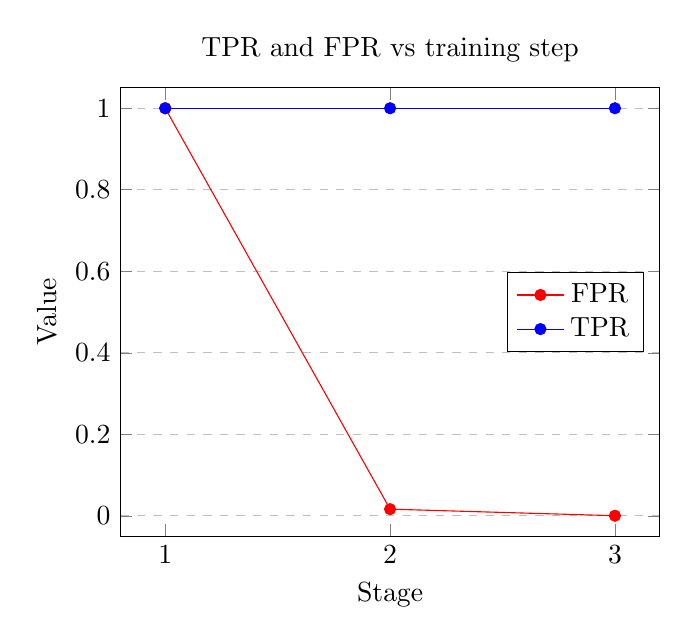
\begin{tikzpicture}
  \begin{axis}[
      title={TPR and FPR vs training step},
      xlabel={Stage},
      ylabel={Value},
      xmin=0.8, xmax=3.2,
      ymin=-0.05, ymax=1.05,
      xtick={1, 2, 3},
      ytick={0, 0.2, 0.4, 0.6, 0.8, 1.0 },
      legend style={at={(0.97,0.5)},anchor=east},
      ymajorgrids=true,
      grid style=dashed,
  ]
  
  \addplot[
      color=red,
      mark=*,
      ]
      coordinates {
        (1,1)(2, 0.0163415)(3, 0.000237497)
      };
  \addlegendentry{FPR}
  
  \addplot[
      color=blue,
      mark=*,
      ]
      coordinates {
        (1,1)(2,1)(3,1)
      };
  \addlegendentry{TPR}
      
  \end{axis}
  \end{tikzpicture}

}
\end{center}

\captionof{figure}{Viola-Jones training results}
\label{fig:vjdarttraininggraph}


\begin{multicols}{3}
    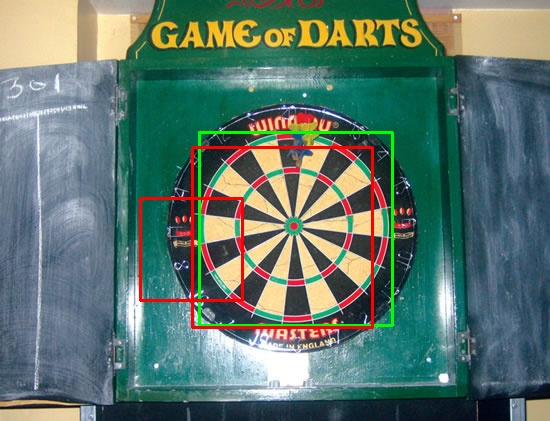
\includegraphics[width=\linewidth]{dart1-dart.jpg}\par
    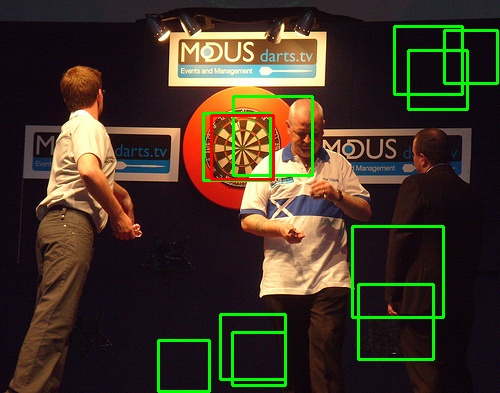
\includegraphics[width=\linewidth]{dart6-dart.jpg}\par
    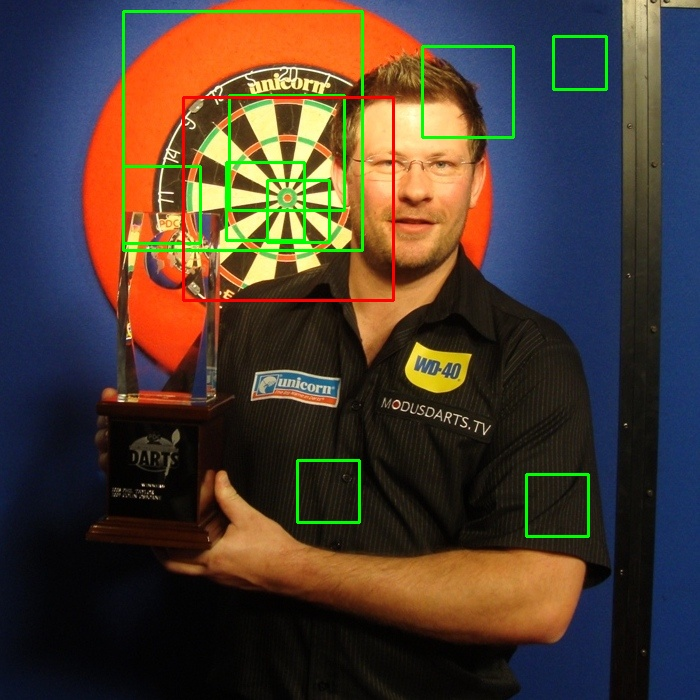
\includegraphics[width=\linewidth]{dart4-dart.jpg}\par
\end{multicols}
\captionof{figure}{Viola-Jones dartboard detection (green) with ground truth (red)}
\label{fig:vjdartsimages}


\begin{center}
\begin{tabular}{ |p{2cm}||p{2cm}|p{2cm}| }
 \hline
 \multicolumn{3}{|c|}{Frontal face detection results} \\
 \hline
 Image name & TPR & F1-SCORE \\
 \hline
 dart1  & 1  & 0.667   \\
 dart2  & 1  & 0.25       \\
 dart3  & 1  & 0.4        \\
 dart4  & 0  & 0          \\
 dart5  & 0  & 0          \\
 dart6  & 1  & 0.182   \\
 dart7  & 0  & 0          \\
 dart8  & 0  & 0          \\
 dart9  & 0  & 0          \\
 dart10 & 0  & 0          \\
 dart11 & 0  & 0          \\
 dart12 & 0  & 0          \\
 dart13 & 0  & 0          \\
 dart14 & 0  & 0          \\
 dart15 & 1  & 0.5        \\
 \hline
 Average& 0.333333  & 0.133232    \\ 
 \hline
\end{tabular}
\captionof{table}{Results of Viola-Jones dartboard detection}
\label{tab:vjdartstable}
\end{center}

The results in Table \ref{tab:vjdartstable} show that the Viola-Jones detector
found one third of the true dartboards in the input images. Reassuringly in
cases where the boards were not detected the Viola-Jones detector often
detected a sub region of the dartboard which can be used in future iterations
of the detector.

However the Viola-Jones algorithm as described in \cite{vj} uses very simple
features (2, 3 or 4 rectangle features). This allows the Viola-Jones algorithm
to be very efficient at detecting certain features in objects such as certain
facial features but is less effective when applied  to more complex objects
such as dartboards. 

The results in Figure \ref{fig:vjdartsimages} also show the detector having
many false positives throughout the images. This contributes to the low F1
score for the results in Table \ref{tab:vjdartstable}.  

These results show that the detector can be effective at detecting the
dartboards repeating pattern. Despite this the TPR remains low as the detected
regions do not meet the required IOU with the true value.  In order to improve
the results the detected regions will have to be filtered to remove many of the
false positives and the resultant bounding regions will have to be shifted to
encompass the whole dartboard. A future detector can build upon the Viola-Jones
reliable detection of the dartboard pattern but will require better detection
of the full dartboard. 

\section{Combining Viola-Jones with hough circle detection}

From the above section it is clear that the Viola Jones detector is not well
suited to detecting full dart boards.  The detector is rarely detecting the
full circular shape of the dart board and has many false positives. However its
effective detection of the dartboards repeating pattern can be combined with a
circle hough transform. This circle hough transform can then be used to remove
detected regions which are not within a circle region This could help reduce
the total number of false positives and thus increase the F1 score of the
detector. Moreover the bounding region from the circle hough transform can be
used as the detected region as this type of detector will be better suited to
detecting the full dart board. The combined steps are as follows:

\begin{itemize}
  \item Run Viola-Jones and hough circles.
  \item For every Viola-Jones results find the maximum IOU with the circles
    from hough. 
  \item If the IOU is greater than a specified threshold (0.25 in this case)
    add the item with the largest area to the set of final results.
\end{itemize} 

This can be represented by the following flow diagram.

\bigskip

\resizebox{\columnwidth}{!}{
  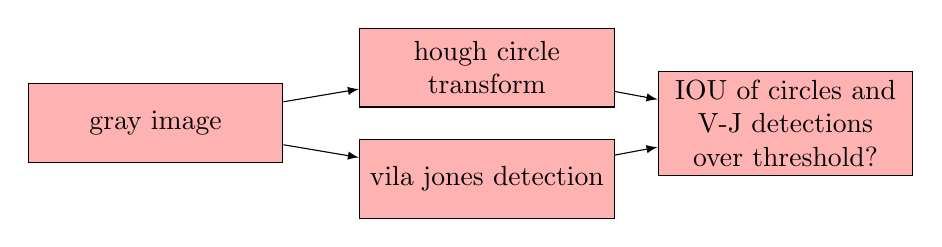
\begin{tikzpicture}[node distance=1cm]
  \tikzstyle{line}=[draw]
  \tikzstyle{process} = [rectangle, minimum width=3cm, minimum height=1cm, text centered, text width=3cm, draw=black, fill=red!30]
  \tikzstyle{decision} = [diamond, minimum width=3cm, text centered, text width=3cm, draw=black, fill=green!30]
  \tikzstyle{sdecision} = [diamond, minimum width=3cm, draw=black, fill=green!30]
  \tikzstyle{arrow}=[draw, -latex]
  
  \node (gray) [process, xshift=3.0cm] {gray image};
  \node (hough) [process, above right of=gray, xshift=3.5cm] {hough circle transform};
  \node (vj) [process, below right of=gray, xshift=3.5cm] {vila jones detection};
  \node (threshold) [process, right of=gray, xshift=7cm] {IOU of circles and V-J detections over threshold?};
  
  \draw [arrow] (gray) -- (hough);
  \draw [arrow] (gray) -- (vj);
  \draw [arrow] (vj) -- (threshold);
  \draw [arrow] (hough) -- (threshold);
  
  \end{tikzpicture}
}

\bigskip

The use of IOU with hough circles resulted in a large reduction in the set of results.
For the required IOU a relatively low threshold was chosen (0.25) as often the
Viola-Jones detector would often find a sub section of the dart board (matching the
expected pattern) but not the circle meaning the relative overlap of the circle
region and this region was small. For this reason the final results used
the maximum of the bounding boxes from the two detectors rather than the
Viola-Jones detector as this was more likely to encompass the full dartboard
and not just a sub section or inner circle. This removed many of the original
Viola-Jones false positives and therefore increased the F1-score dramatically.

One of the limitations of this approach is clear in Figure \ref{fig:hough1results}. On
the right the output image shows one dartboard being successfully detected
while the dartboard to the left is not. This is as a result of the dartboard
being at an angle to the camera. This causes the dartboard's shape to be
elliptical in the gradient image (shown on the left) provided to the Hough circles and thus it is not detected. Figure
\ref{fig:hough2results} shows another limitation of Hough circles, when the dartboard is
block by another object. In this case the inner ring is not obstructed and can
be seen in the output image however the outer ring of the dartboard is
obstructed and therefore the circle is not detected.

\begin{multicols}{2}
  \begin{multicols}{2}
  \centerline{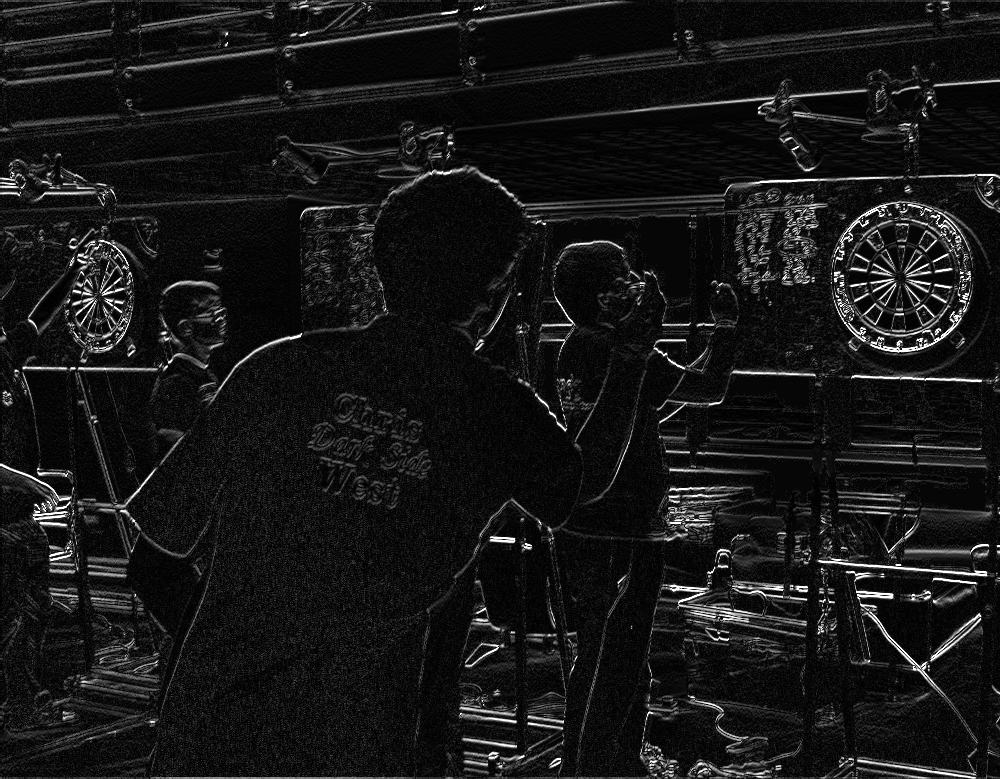
\includegraphics[width=\linewidth]{houghvj/8/gradmag.png}\par}
  \centerline{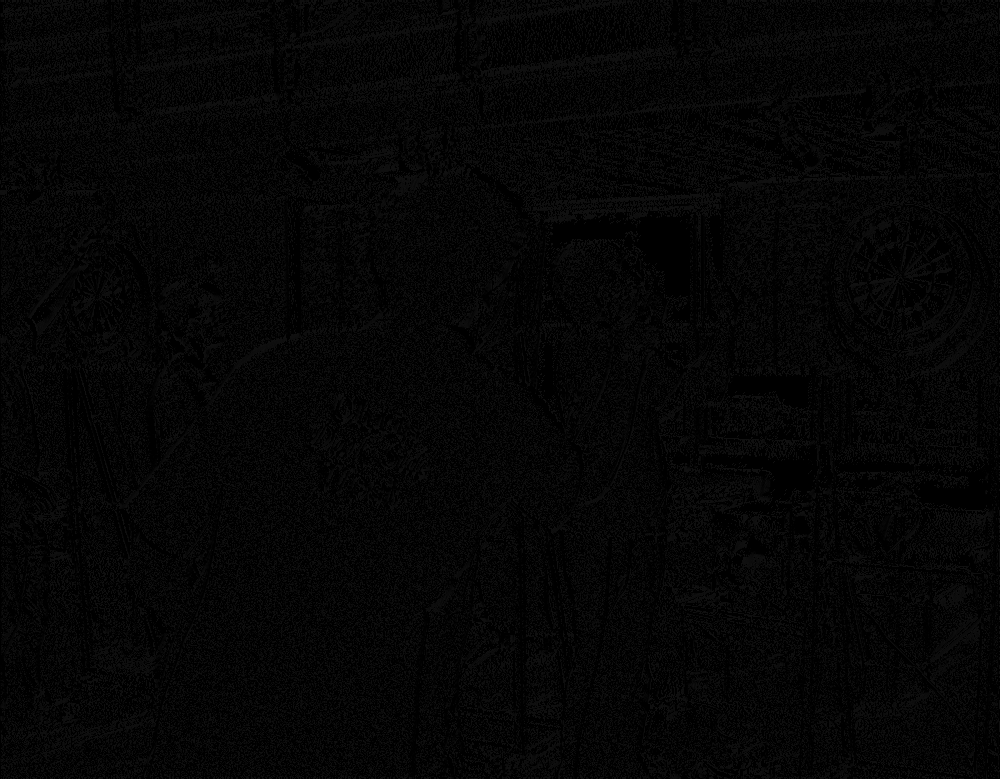
\includegraphics[width=\linewidth]{houghvj/8/graddirection.png}\par}
  \centerline{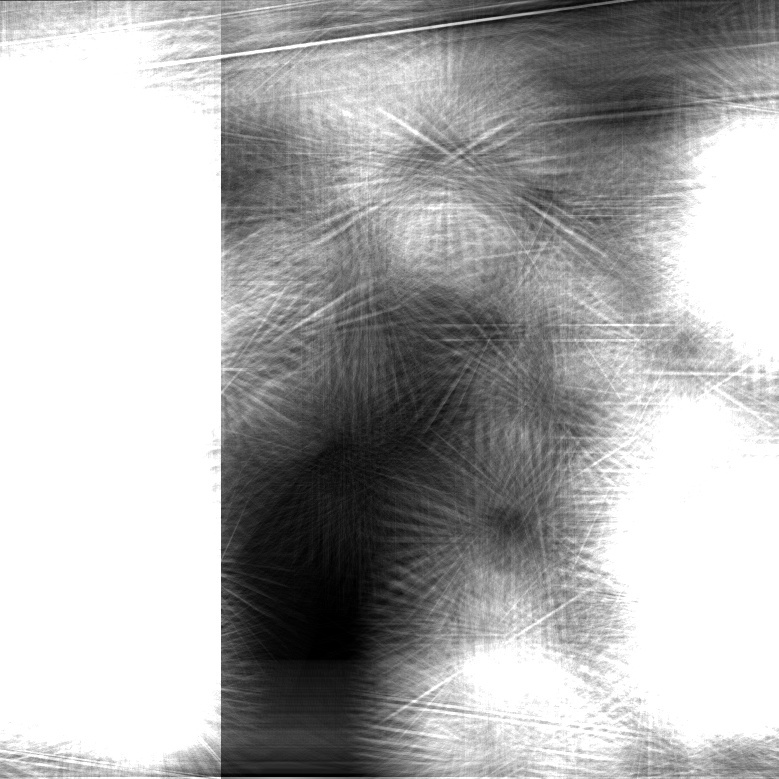
\includegraphics[width=\linewidth]{houghvj/8/cirlce-hough-space.jpg}\par}
  \end{multicols}
  \centerline{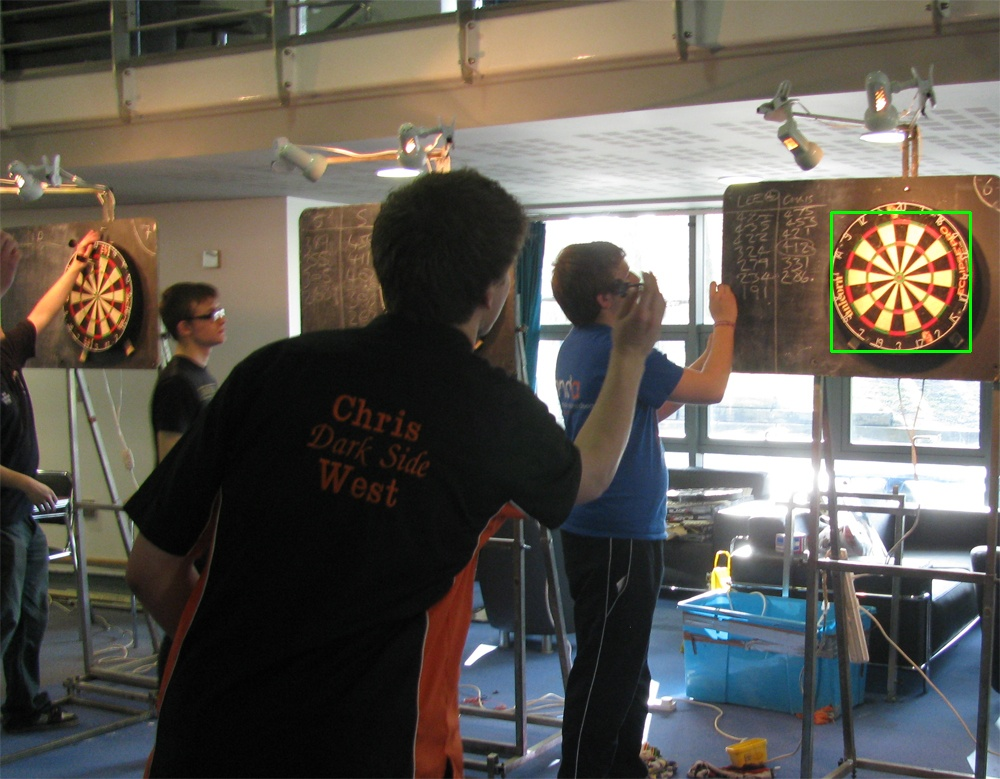
\includegraphics[width=\linewidth]{houghvj/8/final-output.jpg}\par}
\end{multicols}
\captionof{figure}{Hough circle detection on dart8.jpg, showing gradient magnitude, gradient direction, 2D representation of the hough space and the final output respectively}
\label{fig:hough1results}

\begin{multicols}{2}
  \begin{multicols}{2}
  \centerline{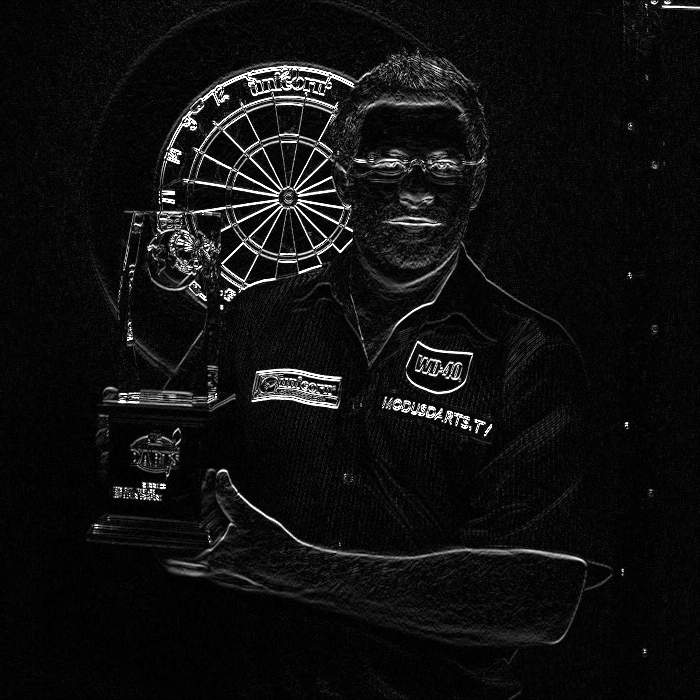
\includegraphics[width=\linewidth]{houghvj/4/gradmag.png}\par}
  \centerline{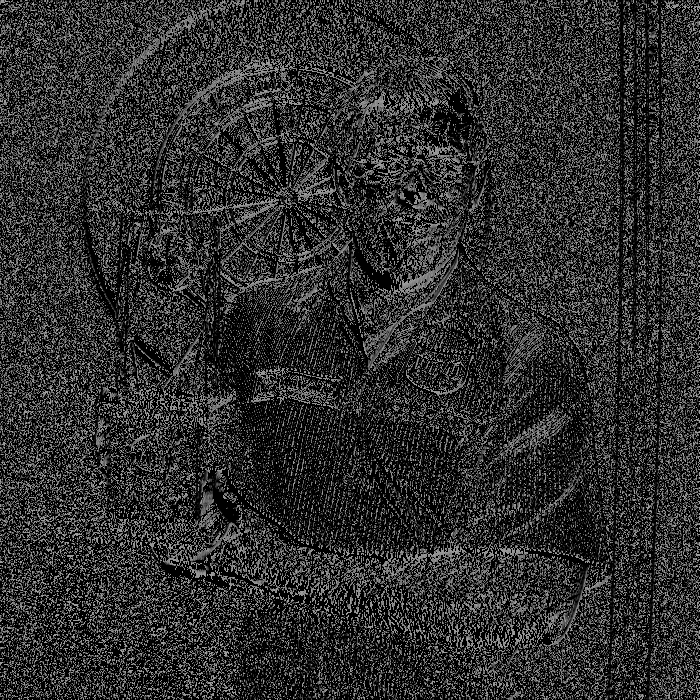
\includegraphics[width=\linewidth]{houghvj/4/graddirection.png}\par}
  \centerline{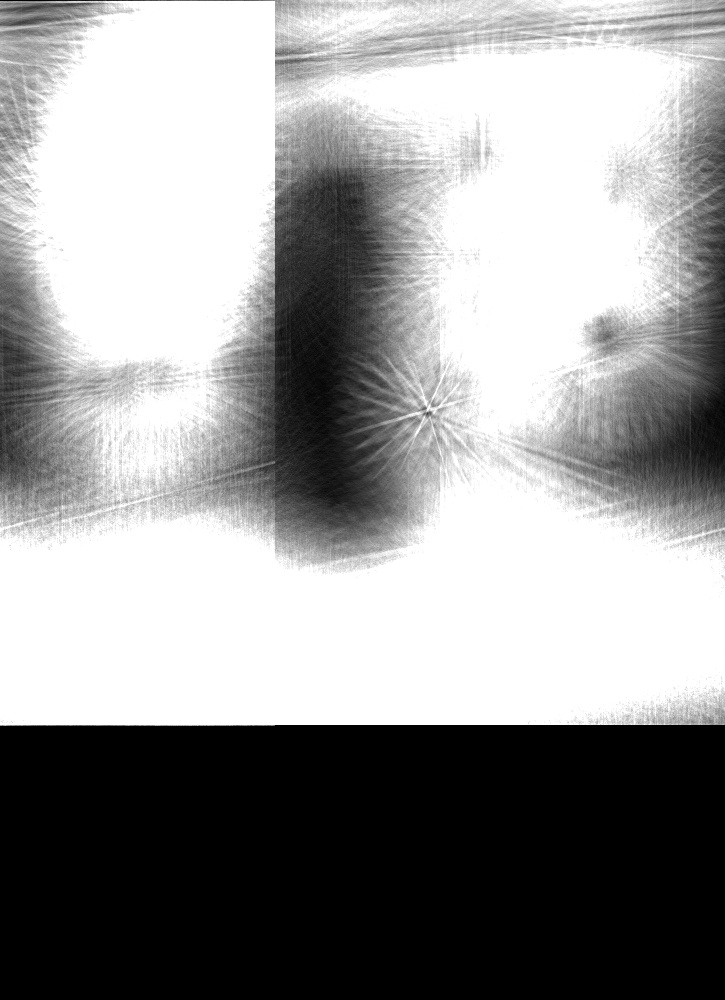
\includegraphics[width=\linewidth]{houghvj/4/cirlce-hough-space.jpg}\par}
  \end{multicols}
  \centerline{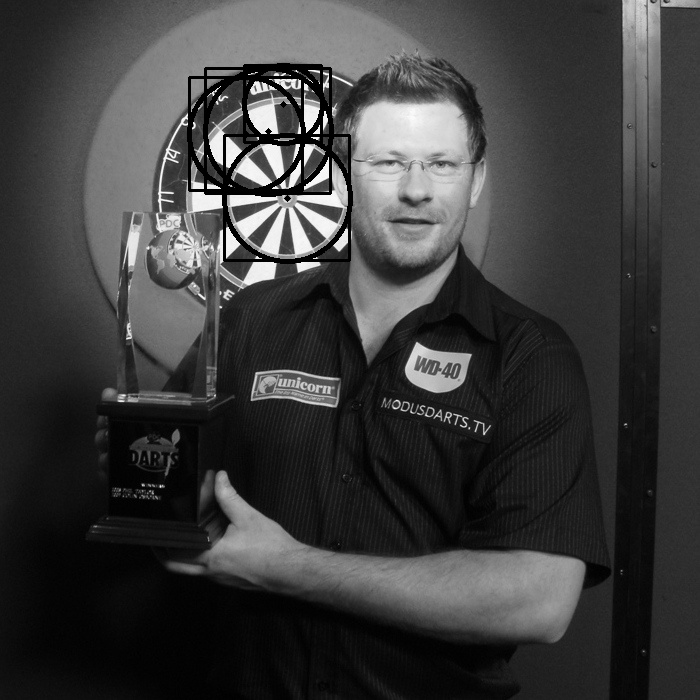
\includegraphics[width=\linewidth]{houghvj/4/cirlce-hough-output.jpg}\par}
\end{multicols}
\captionof{figure}{Hough circle detection on dart4.jpg, showing gradient magnitude, gradient direction, 2D representation of the hough space and the hough circle output respectively}
\label{fig:hough2results}

\begin{center}
\begin{tabular}{ |p{1.3cm}||p{1.3cm}|p{1.3cm}|p{1.3cm}|p{1.3cm}| }
 \hline
 \multicolumn{5}{|c|}{Frontal face detection results} \\
 \hline
 Image name & TPR & F1 & \(\Delta\) TPR & \(\Delta\) F1 \\
 \hline
 dart1  & 1  & 1 & 0 & + 0.333 \\
 dart2  & 1  & 0.5 & 0 & +0.25       \\
 dart3  & 1  & 0.5 & 0 & +0.1       \\
 dart4  & 0  & 0 & 0 & 0         \\
 dart5  & 1  & 1 & +1 & +1         \\
 dart6  & 0  & 0 & -1 & -0.182 \\
 dart7  & 1  & 0.5 & +1 & +0.5         \\
 dart8  & 0.5  & 0.667 & +0.5 & +0.667   \\
 dart9  & 0.5  & 0.4 & +0.5 & +0.4           \\
 dart10 & 0  & 0 & 0 & 0          \\
 dart11 & 0  & 0 & 0 & 0          \\
 dart12 & 0  & 0 & 0 & 0         \\
 dart13 & 1  & 0.4 & +1 & +0.4         \\
 dart14 & 1  & 0.5 & +1 & +0.5         \\
 dart15 & 1  & 0.5 & 0 & 0     \\
 \hline
 Average& 0.6 & 0.364 & +0.267 & +0.264   \\ 
 \hline
\end{tabular}
\captionof{table}{Viola-Jones plus hough circles detection with difference in F1 score and TPR between results in Table \ref{tab:vjdartstable}}
\label{tab:vjhoughdartstable}
\end{center}

Table \ref{tab:vjhoughdartstable} shows the results of the combination of these
two detectors. In 9 of the 15 input images there is an increase in the F1 score
as many more negative regions are now rejected by the extra classification step. 
However in one case (dart6) we do see a reduction in the TPR, this is as a
result of no overlapping circle being found in the region and therefore the
previous Viola-Jones region has been rejected.

In 6 of the 15 input images we see an improvement in TPR. This is as a
result of using the bounding region provided by Hough circles. Since the returned 
region maps to the detected circles it often gave a more accurate
representation of the dartboard region. 

Despite these improvements there were still 5 images where no dartboards were
detected. This suggests an additional method is required to expand the set of
detected values.

The key points for this step are:

\begin{itemize}
  \item The circle detector is ineffective at detecting circles at an angle to the camera or those obstructed by other regions.
  \item The detector has reduced the number of false positives by filtering out the regions which do not overlap circles.
  \item The detector's TPR value has improved by using the circle's bounding regions.
\end{itemize} 


\section{Further Improvements to the Detector}

\subsection{Hough Lines and Combination step}

From the previous results it is clear that the hough circles implementation was
not effective when there were object blocking the dartboard or the dartboard was
at an angle. In order to improve the detector an alternative method is required
which can detect dartboards in these specific conditions. The
proposed approach is as follows:

\begin{itemize}
  \item Run the Viola-Jones detector and Hough circles and filter as before 
  \item Run Hough lines to get a set of lines in the image
  \item For the detected regions from Viola-Jones which are rejected by the
    comparison with hough circles check if there are 3 or more lines which
    intersect inside this region. If so accept the region.
\end{itemize} 

This updates the flow diagram to be as follows:

\resizebox{\columnwidth}{!}{
  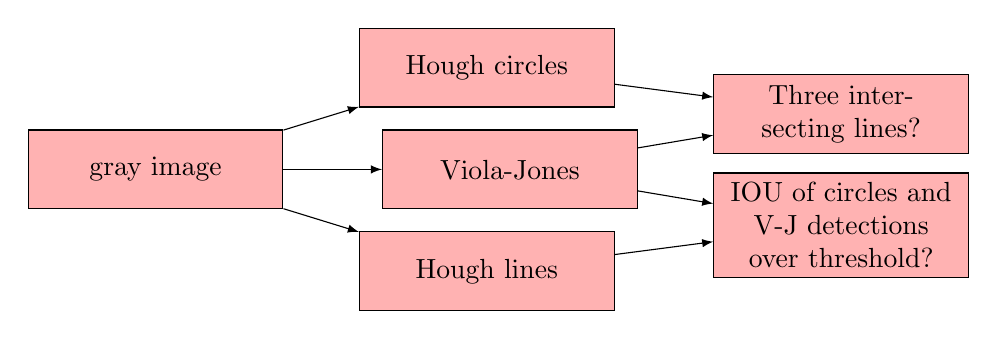
\begin{tikzpicture}[node distance=1cm]
  \tikzstyle{line}=[draw]
  \tikzstyle{process} = [rectangle, minimum width=3cm, minimum height=1cm, text centered, text width=3cm, draw=black, fill=red!30]
  \tikzstyle{decision} = [diamond, minimum width=3cm, text centered, text width=3cm, draw=black, fill=green!30]
  \tikzstyle{arrow}=[draw, -latex]
  
  \node (gray) [process, xshift=3.0cm] {gray image};
  \node (hough) [process, above right of=gray, xshift=3.5cm, yshift=-2cm] {Hough lines};
  \node (vj) [process, right of=gray, xshift=3.5cm] {Viola-Jones};
  \node (lines) [process, below right of=gray, xshift=3.5cm, yshift=2cm] {Hough circles};
  \node (threshold) [process, below right of=vj, xshift=3.5cm] {IOU of circles and V-J detections over threshold?};
  \node (3lines) [process, above right of=vj, xshift=3.5cm] {Three intersecting lines?};
  
  \draw [arrow] (gray) -- (hough);
  \draw [arrow] (gray) -- (vj);
  \draw [arrow] (gray) -- (lines);
  \draw [arrow] (vj) -- (threshold);
  \draw [arrow] (hough) -- (threshold);
  \draw [arrow] (vj) -- (3lines);
  \draw [arrow] (lines) -- (3lines);
  
  \end{tikzpicture}
}

This additional step should allow for those regions not detected by hough
circles an alternative path to being accepted at the cost of potential for a
great number of false positives. The use of Hough lines should allow for the
detection of items at an angle as the lines should still be detectable. Moreover
dartboards which are partially obstructed will still have some visible lines and could therefor still meet the required 3 intersections.

Another key issue with the current detector was multiple regions from within the dartboard being detected. With the addition of Hough circle it was common for both an inner circle and outer circle of the dartboard to be detected. To reduce the number of duplicate detections the following steps were used for each Viola-Jones region:

\begin{itemize}
  \item Find the circle with the greatest IOU with the given Viola-Jones region
  \item If the IOU is greater than the required threshold check all the other circles and find those which have the same (within a given threshold) midpoint
  \item From the circles with the same midpoint add the one with the largest radius to the final results and remove the rest from the list of potential regions (so the inner regions are no accepted later)
\end{itemize}

\begin{center}
\begin{tabular}{ |p{1.3cm}||p{1.3cm}|p{1.3cm}|p{1.3cm}|p{1.3cm}| }
 \hline
 \multicolumn{5}{|c|}{Frontal face detection results} \\
 \hline
 Image name & TPR & F1 & \(\Delta\) TPR & \(\Delta\) F1 \\
 \hline
 dart1  & 1  & 1 & 0 & 0 \\
 dart2  & 1  & 0.667 & 0 & +0.167       \\
 dart3  & 1  & 0.667 & 0 & +0.167      \\
 dart4  & 1  & 0.286 & +1 & +0.286         \\
 dart5  & 1  & 0.5 & 0 & -0.5         \\
 dart6  & 1  & 1 & +1 & +1 \\
 dart7  & 1  & 0.5 & 0 & 0         \\
 dart8  & 0.5  & 0.667 & 0 & 0   \\
 dart9  & 0.5  & 0.286 & 0 & -0.114           \\
 dart10 & 0.333  & 0.182 & +0.333 & +0.182          \\
 dart11 & 0  & 0 & 0 & 0 \\
 dart12 & 0  & 0 & 0 & 0         \\
 dart13 & 1  & 0.333 & +1 & -0.067         \\
 dart14 & 1  & 0.111 & 0 & -0.389        \\
 dart15 & 1  & 1   & 0 & 0     \\
 \hline
 Average& 0.333333  & 0.133232 & +0.289 & +0.298   \\ 
 \hline
\end{tabular}
\captionof{table}{Viola-Jones plus hough circles detection with difference in F1 score and TPR between results in Table \ref{tab:vjdartstable}}
  \label{tab:vjhoughdartslinestable}
  \end{center}

  The results for the updated detector are shown in Table \ref{tab:vjhoughdartslinestable}. In certain cases we see a reduction in the F1 score. This is as a result of the increased number of false positives by allowing an additional set of value to be classified. However this does allow for an increase in total TPR. In some cases this shows that the additional lines check is allowing for some new dartboard to be found.

  However the images in Figure \ref{fig:examplebadhoughlines} show the main limitation of
  this approach. Although the lines clearly pass through those on the dartboard
  the final output does not successfully detect the board. In fact two regions are returned, cutting the dartboard in half. This links to the issue before where the Viola-Jones detector returned a subsection of the detected region. This was solved by using the circle region instead. However when a region is detected by Hough lines there is no mechanism to determine the size of the detected region (only the center point). This means in many cases the new detector fails to improve the TPR of the results as the detected regions do not encompass the whole dartboard.


\begin{multicols}{4}
  \centerline{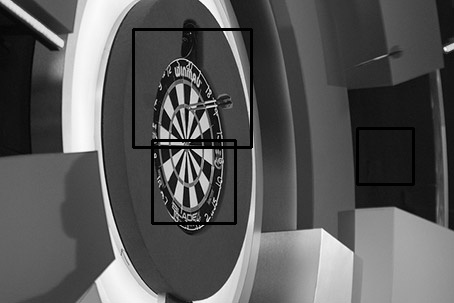
\includegraphics[width=\linewidth]{assets/houghvjlines/12/vj-output.jpg}\par}
  \centerline{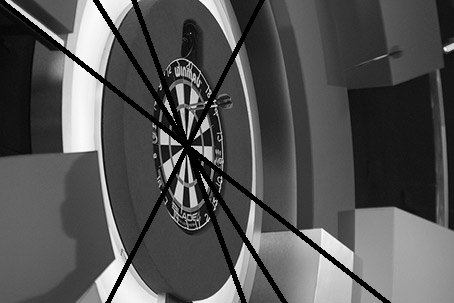
\includegraphics[width=\linewidth]{assets/houghvjlines/12/lines-hough-output.png}\par}
  \centerline{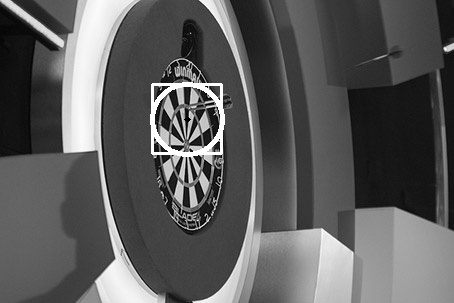
\includegraphics[width=\linewidth]{assets/houghvjlines/12/cirlce-hough-output.jpg}\par}
  \centerline{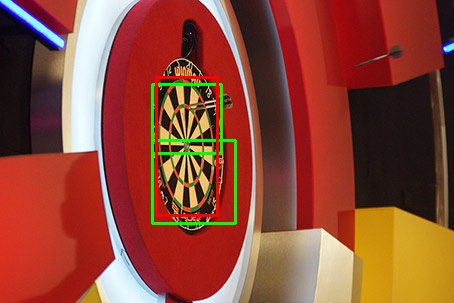
\includegraphics[width=\linewidth]{assets/houghvjlines/12/final-output-true.jpg}\par}
\end{multicols}


\captionof{figure}{Example out of detector using hough lines}
\label{fig:examplebadhoughlines}

\subsection{Future improvement}

Although not pursued in this report, the results above present some clear paths to improve the detector. 
Using a probabilistic Hough line transform, instead of the generic Hough line transform would also return the end points of the detected lines. These line could then both be used to check for the intersecting lines found on the dartboard as well as determine the size and shape of the dartboard. This could then be used to predict the location of the board and remove the duplicate detection from within the dartboard.

Alternatively an Hough ellipse transform could be used. This would allow the detector to find a greater number of the dartboards at an angle and also indicate the true shape of the board in the image. However a hough ellipse requires a 5D Hough space which can be an expensive calculate. Therefore if an efficient algorithm is required probabilistic Hough lines would be the preferred approach.

\end{multicols}

\bibliographystyle{unsrt}
\bibliography{report}

\end{document}
